%! Author = brdvlami
%! Date = 30/04/2024

% Preamble
\documentclass[11pt]{article}
% Packages
\usepackage[all]{nowidow}
\usepackage[english]{babel}
\usepackage{subfloat}
\usepackage{float}
\usepackage[style=ieee, backend=biber]{biblatex}
\addbibresource{abstract_bibliography.bib}
\renewcommand*{\bibfont}{\footnotesize}

\usepackage[small]{titlesec}
\titlespacing*{\section}{0pt}{3ex}{1ex}
\titlespacing*{\subsection}{0pt}{2.5ex}{0.5ex}
\titlespacing*{\subsubsection}{0pt}{3ex}{0.5ex}
\titlespacing*{\paragraph}{0pt}{0.9ex}{1em}
\usepackage{multicol}
\usepackage{caption}
\captionsetup{font=footnotesize}
\usepackage[hyperfootnotes=true]{hyperref}
\usepackage{xcolor}
\hypersetup{
    colorlinks,
    linkcolor={black},
    citecolor={blue!50!black},
    urlcolor={blue!80!black}
}
%\setlength{\parindent}{0em}
\usepackage{geometry}
\geometry{
    a4paper,
    left=15mm,
    right=15mm,
    top=15mm,
    bottom=25mm,
}
\usepackage{graphicx}
\graphicspath{{./figures/}}

\newenvironment{Figure}
{\par\medskip\noindent\minipage{\linewidth}}
{\endminipage\par\medskip}


\newenvironment{Table}
{\par\medskip\noindent\minipage{\linewidth}}
{\endminipage\par\medskip}

\babelhyphenation[english]{Uni-Prot-KB}

% Document
\begin{document}

    \begingroup
    \centering
    \LARGE Unipept 6.0: Fast semi-exact peptide matching with a memory conservative index for UniProtKB\\[1em]
    \large Bram Devlaminck\\[2em]
    \endgroup

    \par\noindent\rule{\linewidth}{.5pt}
    \section*{Abstract}\label{sec:test-section}
    Unipept is an ecosystem of software tools developed for fast metaproteomics data analysis.
    In the past few years, Unipept has been optimized for tryptic peptide search, with a slow workaround for peptides with missed cleavages.
    Unipept 6.0 introduces a new index structure that allows ultra-fast peptide matching for arbitrary peptides.
    This now makes Unipept applicable in domains where trypsin is not the protease of choice, and also removes the performance penalty when dealing with missed cleavages.
    In addition to these advancements, Unipept 6.0 maintains its superior performance compared to similar tools, ensuring efficient and accurate metaproteomics data analysis.
    \par\noindent\rule{\linewidth}{.5pt}

    \begin{multicols}{2}
%        \raggedcolumns
        \section{Introduction}\label{sec:introduction}
        Traditionally, trypsin is the most used protease in the (meta)proteomics field.
        Unipept~\cite{unipept_desktop, unipept_api, unipept_4, unipept_orig, unipept_tutorial, unipept_web, unipept_cli, unipept_desktop_2} was specifically developed with this in mind.
        As a result, Unipept uses an index structure where the UniProtKB~\cite{UniprotKB} database is preprocessed by splitting every protein according to the cleavage pattern created by trypsin.
        This allows Unipept to precompute the Lowest Common Ancestor (LCA) for every tryptic peptide digestion from UniProtKB\@.
        This approach has proven its efficiency in the past few years, but also has its limitations.

        From time to time, trypsin will miss a cleavage position, creating a so-called missed cleavage.
        Peptides with such missed cleavages will not be present in the current Unipept index, since Unipept assumes there are no missed cleavages.
        To solve this problem, a solution was retro-fitted to handle these missed cleavages.
        When this option is selected, Unipept scans the input peptides for missed cleavage positions, splits the peptides and perform separate lookups for every tryptic fragment.
        The resulting sets of protein matches are intersected, which delivers a set of possible protein matches.
        Every protein in this set is brute-force scanned to ensure that the original peptide is present, and not only its separate tryptic fragments.
        Finally, the LCA of the found proteins is calculated on the fly.
        All these extra steps, including the on the fly calculation of the LCA, have a significant impact on performance.

        A second disadvantage of the current Unipept index, is the inability to process non-tryptic peptides.
        Similar to peptides with missed cleavages, these will not be present in the index, but no workaround exists in this case.

        This restriction has not been a significant issue since Unipept was originally created for metaproteomics, where trypsin is widely used.
        However, other fields such as immunopeptidomics~\cite{immunopeptidomics} frequently work with non-tryptic peptides.
        Tools such as MS$^2$Rescore~\cite{ms2rescore} and MS$^2$PIP~\cite{ms2pip} have been adding support for immunopeptidomics research.
        As we aspire to broaden the use cases of Unipept, adding support for these upcoming research fields is important.
        This requires a new index structure with the following properties:

        \begin{enumerate}
            \item For every peptide (tryptic or non-tryptic), all protein matches in UniProtKB should be found.
            \item The maximum memory usage when building the index for the complete UniProtKB database should be around 1 to 2 TB due to current hardware limitations.
            \item Search performance should be on par with Unipept 5.x for tryptic peptides.
            \item The new index should facilitate all Unipept 5.x features.
        \end{enumerate}

        In short, we want an index that does not remove any of the features from Unipept 5.x, while eliminating the restriction that only tryptic peptides can be found efficiently.
        This also means that our new index will need to provide a way to equate the amino acids isoleucine and leucine, as this is a core feature~\cite{unipept_orig}.


        \section{Methods}\label{sec:methods}
        At the core of our new index structure is a suffix array.
        This suffix array can be build using the libdivsufsort~\cite{libdivsufsort} or libsais~\cite{libsais} library.
        Both provide a linear time algorithm with a $5n + O(1)$ memory complexity, where $n$ is the size of the text that needs to be indexed.
        Depending on the used text, one implementation is faster than the other.

        \subsection{Sparse Suffix Arrays}
        While a complete suffix array delivers the best performance, the index itself is large.
        The size of the suffix array can be reduced by introducing a sampling step to create a so-called sparse suffix array (SSA).
        This variant of a suffix array only stores every $k$-th suffix of the input text.
        This results in an SSA which is only $\frac{1}{k}$ of the original suffix array size.
        The disadvantage of using an SSA is that it becomes impossible to search for peptides having less than $k$ amino acids, and that searching in general becomes slower.
        This trade-of does not introduce any problem, since Unipept already limits the search searching to peptides with 5 or more amino acids.
        This restriction was introduced to improve performance, while losing a minimum amount of information as short peptides occur in a lot of proteins.
        Searching short peptides yields extremely generic functional and taxonomic analysis results, which is not very informative.

        \subsection{Equating Isoleucine and Leucine}
        Our solution to equate isoleucine and leucine consists of two parts.
        Firstly, we don't index the original text, but a slightly modified version.
        We replace every occurrence of leucine by isoleucine, which essentially equates them during the construction of the suffix array.
        During the search, we perform the same translation on every peptide.
        As a result, we find every match with I and L equated.
        This search is performed using the original, unmodified text.
        This is important, since the original text is needed in an additional second step if we don't want to equate I and L\@.

        During this second step, we filter away unwanted matches from the first step.
        This is achieved by checking every I and L location in the original, unmodified peptide with the matching amino acid in the original, unmodified text.
        A mismatch indicates that I and L were wrongfully equated.
        Only the I and L locations have to be checked since the suffix array search already ensures that all other characters match in the original text.

        \subsection{Analyses}
        Our solution performs the functional and taxonomic analysis at runtime.
        While it would be advantageous to precompute this, the suffix array and text do not contain enough information to do this.
        This is a trade-off we made during development between optimal memory usage and speed.

        \subsection{Maximum Matches}
        A single peptides can occur in thousands of proteins.
        Because of this, performing the analyses at runtime can become slow.
        Furthermore, the analyses for such peptides yields very a generic result in most cases.
        More precisely, earlier research by the Unipept team~\cite{unipept_cutoff} has shown that out the 1.3 billion tryptic peptides in UniProtKB 2023\_03, only around 13\thinspace000 had more than 10\thinspace000 matches. % TODO: cite research
        From these 13\thinspace000 peptides, 95\% of the peptides had \texttt{root} as LCA\@.
        This allows, with minimal loss of information, to assume that every peptide with more than 10\thinspace000 matches has \texttt{root} as LCA\@.
        Additionally, this limits the amount of information returned per query.

        \section{Results}\label{sec:results}
        Three main factors are considered during testing.
        The memory usage and speed during construction, the resulting index size while hosting, and search performance.

        \subsection{Constructing the Index}
        Constructing a suffix array for the complete UniProtKB database (release 2024\_01) requires around 735 GB of RAM and 5 hours of computing time using the libdivsufsort library.
        Because of the high memory needs, we use the HPC of Ghent University, where the high-memory cluster has 16 nodes with each 2\times 64-core AMD EPYC 7773X (Milan-X @ 2.2 GHz) and 940 GB of RAM\@.
        We use one core of a single node, since the construction phase is single threaded.
        The resulting suffix array is around 700 GB in size (+ an additional 88 GB for the text).
        Our goal is to host this new index on Unipept servers, which have around 0.5 TB of memory available.
        To make this possible, we immediately perform a sampling phase with sparseness factor $k = 3$ at the end of the construction process on the HPC\@.
        This results in a reduced index size of $\frac{700}{3} + 88 \approx 322$ GB\@.
        Next to this peptide search index, Unipept needs extra information (such as the UniProt accession number, NCBI taxon ID and functional annotations per protein) to perform the provided analyses.
        This results in another 25 GB of RAM needed.
        Figure~\ref{fig:uniprot_memory_treemap} visualizes the size of each component of the resulting index.

        \begin{Figure}
            \centering
            \resizebox{\textwidth}{!}{
                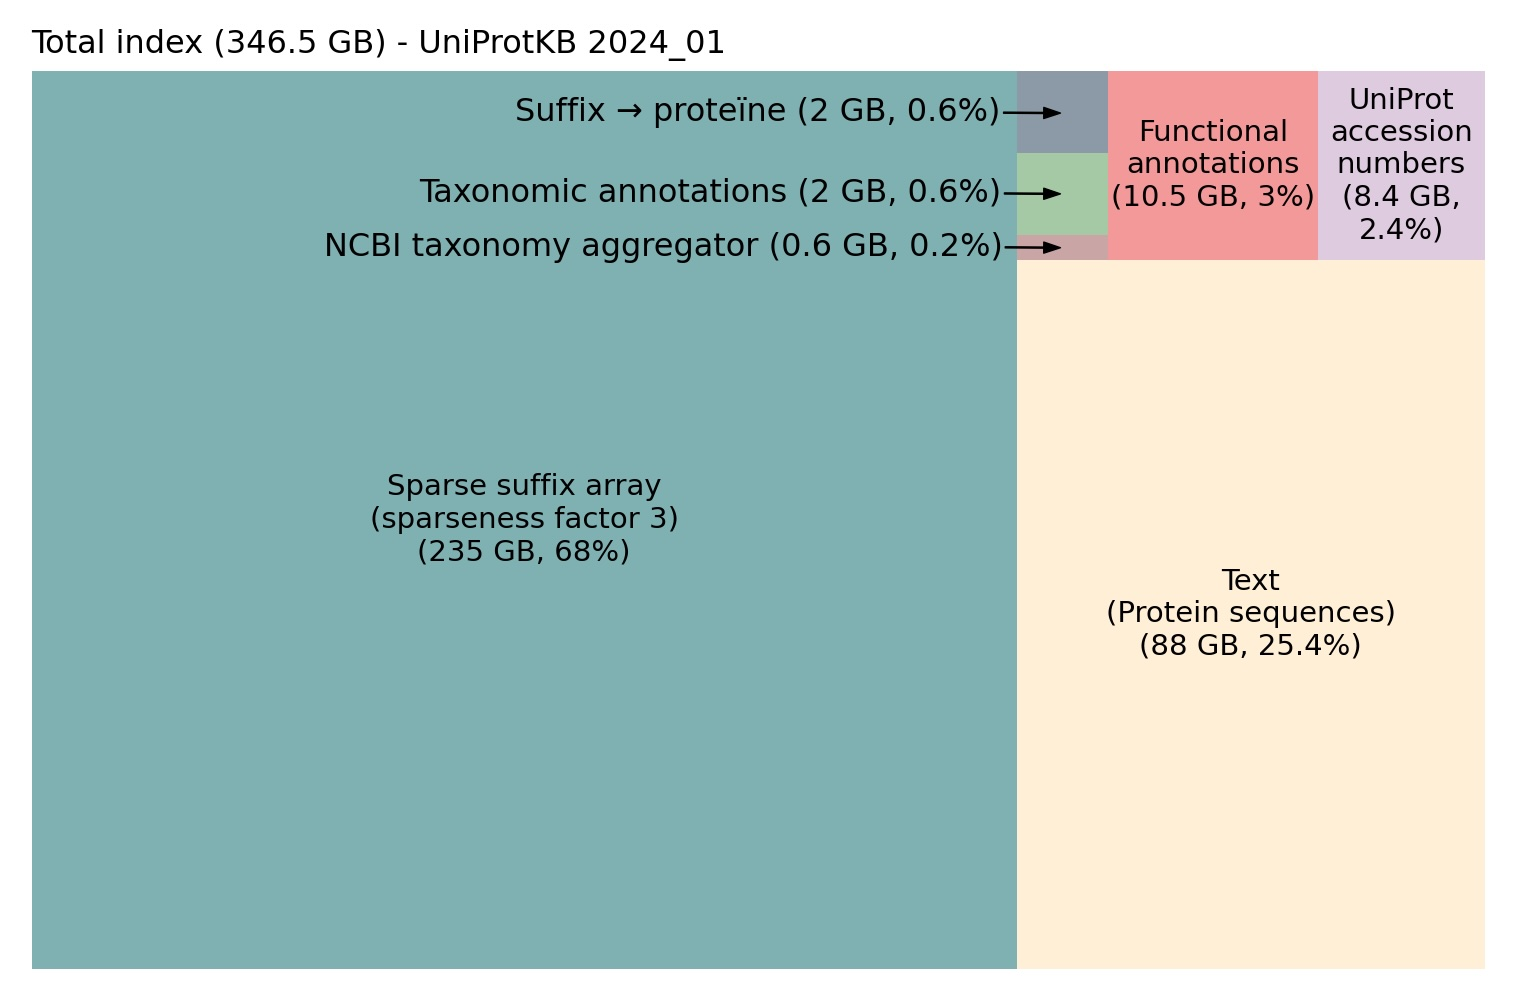
\includegraphics{uniprot_memory_treemap}
            }
            \captionof{figure}{Visualisation of the size of each component of the new Unipept index for UniProtKB 2024\_01.}
            \label{fig:uniprot_memory_treemap}
        \end{Figure}

        \subsection{Querying the Index}
        Unipept 6.x supports two types of search.
        Most importantly, we can efficiently search all matches and perform the taxonomic and functional analyses at runtime.
        Since the analyses is executed at runtime, we already have all the information per matched protein.
        With Unipept 6.x we provide search without analyses as a separate option.
        This was not possible with Unipept 5.x since the analyses were precomputed and retrieving all information per protein was too slow.
        Both search options in Unipept 6.x perform similar.
        Surprisingly, the first option is slightly faster.
        This is caused by the additional information per protein that needs to be serialized, since the functional annotations are not aggregated.
        In this section we only discuss the search with analyses, since this is what Unipept 5.x supports and the other search option performs very similar.

        \paragraph{Missed cleavages}
        To evaluate the peptide search performance we use 6 files with around 25\thinspace000 peptides each.
        These are samples from the SIHUMIx experiment~\cite{SIHUMI_frequently_used, SIHUMI_first_introduction}, where trypsin is used as a protease.
        This means that as well as tryptic peptides, there are also peptides present with naturally occurring missed cleavages.
        Figure~\ref{fig:new_vs_old_unipept} shows the execution time for both Unipept 6.x and 5.x.
        To make the comparison as fair as possible, the \textit{filter duplicate peptides} setting is turned off, and \textit{advanced missed cleavage handling} is turned on.
        This ensures that both indices search every peptide from the input file (including duplicates and peptides with missed cleavages).
        Unipept 6.x is 10 to 100 times faster, which clearly removes the performance penalty that was currently associated with handling missed cleavages.
        Note that the Unipept 5.x index will not find peptides resulting from using a different protease, whereas this makes no difference for the Unipept 6.x index.

        \paragraph{Tryptic peptides}
        A second interesting case to consider is when searching strictly tryptic peptides.
        In that case, missed cleavage handling can be disabled in Unipept 5.x, which significantly improves the performance.
        Figure~\ref{fig:new_vs_old_unipept_tryptic} visualizes the processing time for 100\thinspace000 tryptic peptides.
        It is clear that the performance is comparable when I and L are equated, while Unipept 5.x is around a third faster than Unipept 6.x when I and L are not equated.

        Furthermore, it is also clear that the extra filtering step, when I $\neq$ L, has a performance impact in the new index.
        This effect was not visible in Figure~\ref{fig:new_vs_old_unipept}, where the reverse seems to be visible.
        However, this reverse effect can be explained by the fact that searching with I = L finds more matches, which requires more output to be serialized to a JSON file.
        When searching for larger files, there is proportionally more time spent in the search phase, which compensates for the longer serialization time.

        \begin{Figure}
            \centering
            \resizebox{\textwidth}{!}{
                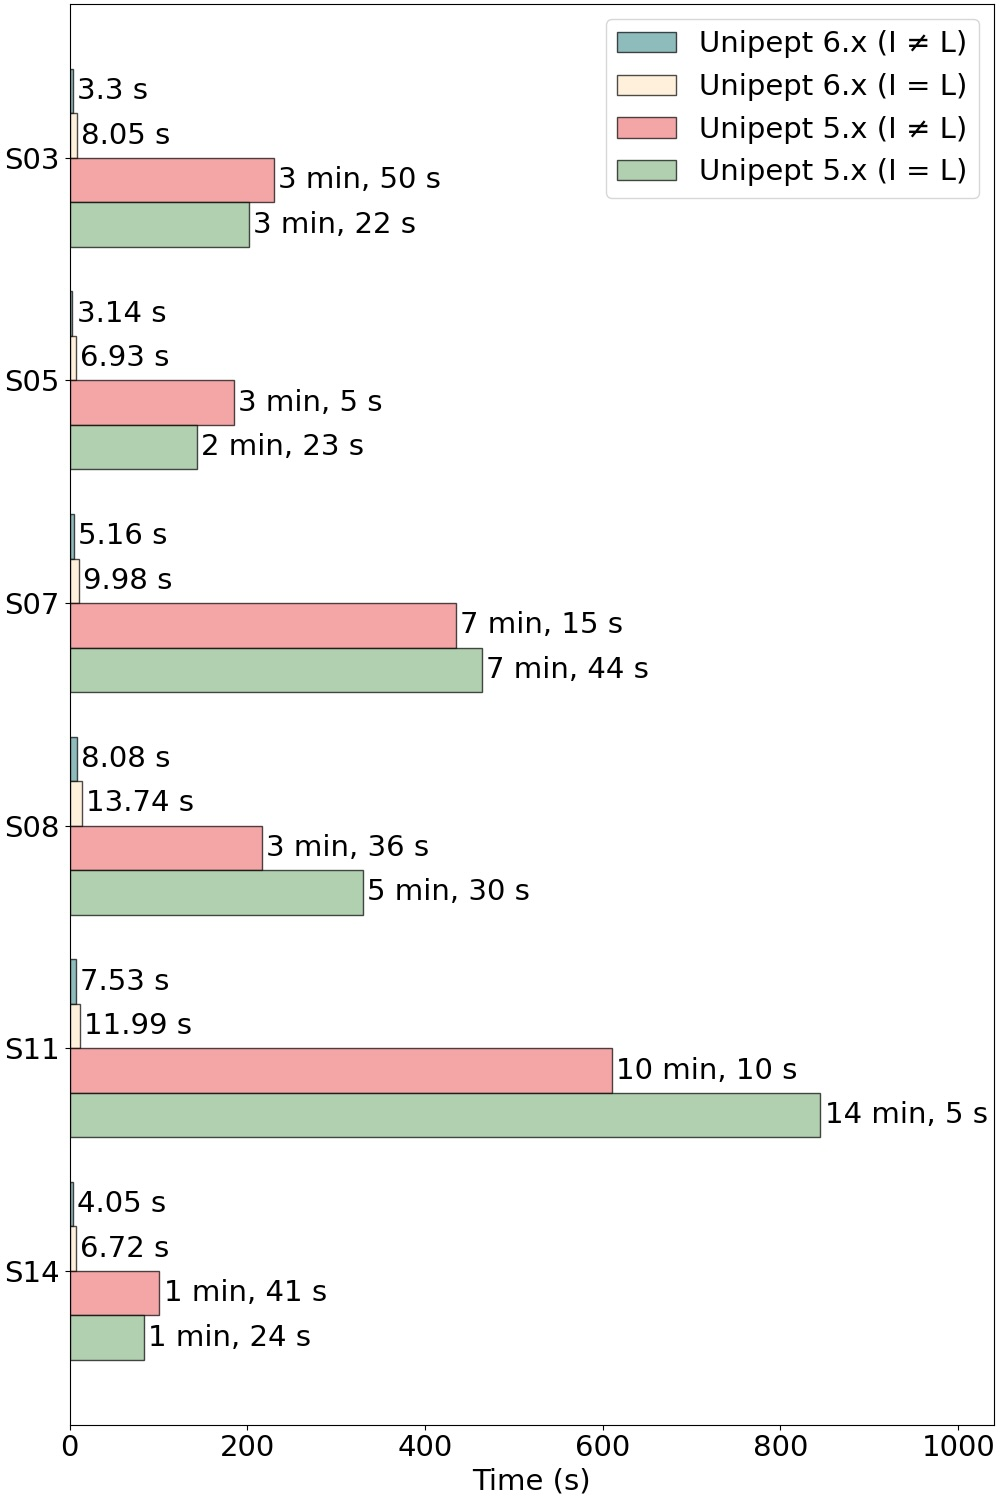
\includegraphics{new_vs_old_unipept}
            }
            \captionof{figure}{Execution time for Unipept 6.x and Unipept 5.x while processing different SIHUMIx samples. Each sample consists of approximately 25\thinspace000 peptides. Unipept 5.x searches with the \textit{filter duplicate peptides} setting turned off, and \textit{advanced missed cleavage handling} turned on. This way both indices search all peptides (included duplicates), and missed cleavages are handled by both. The used test files can be found in our GitHub repository \url{https://github.com/BramDevlaminck/Thesis_benchmarkdata/tree/master/SIHUMI}}
            \label{fig:new_vs_old_unipept}
        \end{Figure}

        \begin{Figure}
            \centering
            \resizebox{\textwidth}{!}{
                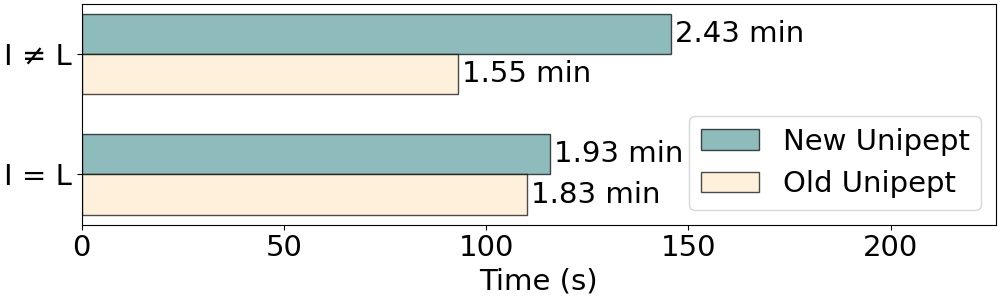
\includegraphics{new_vs_old_unipept_tryptic}
            }
            \captionof{figure}{Processing time for 100\thinspace000 tryptic peptides for Unipept 6.x and 5.x. This is the best case scenario for Unipept 5.x where missed cleavages are \textbf{not} handled.}
            \label{fig:new_vs_old_unipept_tryptic}
        \end{Figure}

        \section{Other Tools}\label{sec:comparison}
        Tools such as the Uniprot peptide search tool~\cite{uniprot_search_site, uniprot_search_paper}, the Expasy ScanProsite tool~\cite{scanprosite} and Unipept 5.x all have the possibility to find matches in the UniProtKB database.
        In this section we compare the performance and feature sets of alternative tools with Unipept 6.x.
        Because of the poor performance of some of these tools, we limited testing to the randomly chosen tryptic peptide \texttt{ISPAVLFVIVILAVLFFISGLLHLLVR}.
        Unipept 6.x uses the settings described above and finds all matches for the test peptide in less than 5 ms.

        In terms of features, the UniProt peptide search tool is identical to Unipept 6.x.
        They both find all matches in UniProtKB, and have the option to equate I and L\@.
        The only difference is their performance.
        Searching the test peptide in Unipept 6.x only takes a few milliseconds, whereas the UniProt tool takes a few seconds up to multiple minutes.

        The Expasy ScanProsite tool takes another approach.
        They provide a wide range of options for inexact matching.
        They call these motifs, and these are comparable to regular expressions where the user can use wildcards, character classes and even negations.
        The other major difference is that this tool does not use the whole UniProtKB database.
        Only the proteins that are part of a reference genome are indexed, which means only around one third of the complete UniProtKB database is indexed.
        Lastly, searching the test peptide takes around 5 minutes.
        As expected, since not the whole UniProtKB database is indexed, only a subset of the matches is found.

        The last major tool we compare with, is Unipept 5.x.
        Unipept 6.x supports all options provided by Unipept 5.x, while removing the restriction that only tryptic peptides can be searched.
        This means that all non-tryptic peptides will result in 0 protein matches in Unipept 5.x, whereas Unipept 6.x will find all protein matches that are in UniProtKB\@.
        Searching the test peptide took less than 5 ms, and found the same matches because our test peptide is tryptic.
        It is important to note though, if we had chosen a non-tryptic peptide we would not have found any matches.
        Table~\ref{tab:tool_comparison} gives an overview of the described differences between the tools.

        \begin{Table}
            \centering
            \resizebox{\textwidth}{!}{
                \begin{tabular}{ l l l l l }
                    & UP6      & UPS          & ESP        & UP5            \\
                    \hline\hline
                    Used proteins    & all      & all          & ref. prot. & all            \\
                    Approx. match    & [IL]     & [IL]         & flexible   & [IL]           \\
                    Time             & $<$ 5 ms & 1 s - 20 min & 5 min      & $<$ 5 ms       \\
                    Searchable pept. & all      & all          & all        & $\sim$ tryptic \\
                    \hline
                \end{tabular}
            }
            \captionof{table}{Comparison of Unipept 6.x (UP6), UniProt Peptide Search (UPS) tool, Expasy ScanProSite (ESP) tool and Unipept 5.x (UP5) index. \texttt{[IL]} in the approximate matching row means that only I and L can be equated, while \texttt{$\sim$ tryptic} in the searchable peptide row means that only tryptic peptides or tryptic peptides with missed cleavages can be found.}
            \label{tab:tool_comparison}
        \end{Table}

        \section{Conclusion}\label{sec:discussion}
        With a new index structure at the heart of Unipept 6.x, we have broadened Unipept's possible use cases.
        The new index structure makes searching peptides with missed cleavages around 10 to 100 times faster, while adding the possibility to search arbitrary peptides, regardless of the used protease, without any performance difference.
        In our benchmarks, Unipept 6.x strongly outperforms its closest competitors at finding all occurrences for an arbitrary peptide longer than 2 amino acids in UniProtKB\@.

        Our new index is optimized for search with leucine and isoleucine equated to each other.
        This corresponds to the default search configuration of Unipept.
        However, searching with I $\neq$ L only introduces a small performance penalty.
        For smaller batches of peptides, the time needed to serialize the extra matches even outweighs the extra time spent during the search phase itself.

        Another advantage of the new index is that there are no extra steps required to retrieve the NCBI taxon ID for each matched protein.
        Extra steps are required in Unipept 5.x to retrieve all the individual taxon IDs, with a significant impact on the performance.
        This restriction created a bottleneck in the new Peptonizer2000 tool~\cite{pep_gm} that has now been removed.

        The main disadvantage of Unipept 6.x compared to Unipept 5.x is that searching tryptic peptides is slightly slower than before, especially when searching with I $\neq$ L\@.
        This slowdown is introduced by taxonomic analyses performed at runtime, whereas these could all be precalculated with the old index that was restricted to tryptic peptides.
        However, this slowdown is limited and acceptable.
        Especially when keeping in mind that real life samples always have some missed cleavages, which would not have been found before, without a performance hit.

        \section{Future Work}
        The Unipept 6.x index meets the pre-established requirements, but still leaves room for improvement in several areas.

        A significant part of the current computation time is invested in performing the taxonomic and functional analyses at runtime.
        Modifying the new index to support pre-calculation of these analyses, while still maintaining a peak memory usage which is manageable would drastically improve the performance.
        Enhanced suffix arrays (ESA) could facilitate this, but require more memory.

        Another area of improvement is the index size itself.
        The index size could be reduced even more by making the text and suffix array more compact.
        Both of these components don't utilize all the bits from the allocated bytes.
        The suffix array only needs 37 of the 64 bits used by every entry, while the text only needs 5 bits out of each byte per character.
        This could reduce the total index size from 346 GB to around 215 GB\@.
        However, this would introduce extra steps to decode every access to any of these data structures.
        This could introduce a non-negligible performance penalty.

        Another option to reduce the index size is by switching to a completely different index structure.
        Both the FM-index and R-index have shown promising results in this respect.

        Lastly, Unipept does not perform any form of inexact matching, except for equating I and L\@.
        Introducing inexact matching into Unipept could allow us to deal with small mutations or variations introduced during the transformation from mass spectrum to peptide.
        Possible interesting routes to explore are regex matching using suffix arrays~\cite{regex_sa}, or inexact matching using bidirectional FM-indices.
        \printbibliography
    \end{multicols}


\end{document}